\documentclass[cs4size,a4paper]{ctexart}   
%==================== 数学符号公式 ============
\usepackage{amsmath}                 % AMS LaTeX宏包
\usepackage[style=1]{mdframed}
\usepackage{amsthm}
\usepackage{amsfonts}
\usepackage{mathrsfs}                % 英文花体字 体
\usepackage{bm}                      % 数学公式中的黑斜体
\usepackage{bbding,manfnt}           % 一些图标,如 \dbend
\usepackage{lettrine}                % 首字下沉,命令\lettrine
\def\attention{\lettrine[lines=2,lraise=0,nindent=0em]{\large\textdbend\hspace{1mm}}{}}
\usepackage{longtable}
\usepackage[toc,page]{appendix}
\usepackage{geometry}                % 页边距调整
\geometry{top=3.0cm,bottom=2.7cm,left=2.5cm,right=2.5cm}
%====================公式按章编号==========================
\numberwithin{equation}{section}
\numberwithin{table}{section}
\numberwithin{figure}{section}
%================= 基本格式预置 ===========================
\usepackage{fancyhdr}
\pagestyle{fancy}
\fancyhf{}  
\fancyhead[C]{\zihao{5}  \kaishu 机\ 器\ 学\ 习\ 结\ 课\ 报\ 告}
\fancyfoot[C]{~\zihao{5} \thepage~}
\renewcommand{\headrulewidth}{0.65pt} 
%\CTEXsetup[format={\centering\bfseries\zihao{-2}}]{section}
\ctexset{
    section={format={\centering\bfseries\zihao{-2}}},
    subsection={nameformat={\bfseries\zihao{3}}},
    subsubsection={nameformat={\bfseries\zihao{4}}}
}
%================== 图形支持宏包 =========================
\usepackage{subfigure}
\usepackage{graphicx}                % 嵌入png图像
\usepackage{color,xcolor}            % 支持彩色文本、底色、文本框等
\usepackage{hyperref}                % 交叉引用
\usepackage{caption}
\captionsetup{figurewithin=section}
%==================== 源码和流程图 =====================
\usepackage{listings}                % 粘贴源代码
\usepackage{xcolor}
\usepackage{color}
\definecolor{dkgreen}{rgb}{0,0.6,0}
\definecolor{gray}{rgb}{0.5,0.5,0.5}
\definecolor{mauve}{rgb}{0.58,0,0.82}
\usepackage{xcolor}
\lstset{
    %行号
    numbers=left,
    %背景框
    framexleftmargin=8mm,
    frame=none,
    %背景色
    %backgroundcolor=\color[rgb]{1,1,0.76},
    backgroundcolor=\color[RGB]{245,245,244},
    %样式
    keywordstyle=\bf\color{blue},
    identifierstyle=\bf,
    numberstyle=\color[RGB]{0,192,192},
    commentstyle=\it\color[RGB]{0,96,96},
    stringstyle=\rmfamily\slshape\color[RGB]{128,0,0},
    %显示空格
    showstringspaces=false
}


%--------------------
\hypersetup{hidelinks}
\usepackage{booktabs}  
\usepackage{shorttoc}
\usepackage{tabu,tikz}
\usepackage{float}

\usepackage{multirow}



\tabcolsep=1ex
\tabulinesep=\tabcolsep
\newlength\tikzboxwidth
\newlength\tikzboxheight
\newcommand\tikzbox[1]{
    \settowidth\tikzboxwidth{#1}
    \settoheight\tikzboxheight{#1}
    \begin{tikzpicture}
        \path[use as bounding box]
            (-0.5\tikzboxwidth,-0.5\tikzboxheight)rectangle
            (0.5\tikzboxwidth,0.5\tikzboxheight);
        \node[inner sep=\tabcolsep+0.5\arrayrulewidth,line width=0.5mm,draw=black]
            at(0,0){#1};
    \end{tikzpicture}%
}

\makeatletter
\def\hlinew#1{
    \noalign{\ifnum0=`}\fi\hrule \@height #1 \futurelet
    \reserved@a\@xhline
}
   
\newcommand{\tabincell}[2]{\begin{tabular}{@{}#1@{}}#2\end{tabular}}%

\usepackage{subfigure}

\usepackage{ifthen}


\usepackage{graphicx} 
\newcommand{\HRule}{\rule{\linewidth}{0.5mm}}

\newtheorem{Theorem}{定理}
\newtheorem{Lemma}{引理} 
%%使得公式随章节自动编号
\makeatletter
\@addtoreset{equation}{section}
\makeatother
\renewcommand{\theequation}{\arabic{section}.\arabic{equation}}

%-------------------------
	
\usepackage{pythonhighlight}
\usepackage{tikz}                    
\usepackage{tikz-3dplot}
\usetikzlibrary{shapes,arrows,positioning}
%===================   正文开始    ===================
\begin{document}
\bibliographystyle{gbt7714-2005}     %论文引用格式
%===================  定理类环境定义 ===================
\newtheorem{example}{例}              % 整体编号
\newtheorem{algorithm}{算法}
\newtheorem{theorem}{定理}            % 按 section 编号
\newtheorem{definition}{定义}
\newtheorem{axiom}{公理}
\newtheorem{property}{性质}
\newtheorem{proposition}{命题}
\newtheorem{lemma}{引理}
\newtheorem{corollary}{推论}
\newtheorem{remark}{注解}
\newtheorem{condition}{条件}
\newtheorem{conclusion}{结论}
\newtheorem{assumption}{假设}
%==================重定义 ===================
\renewcommand{\contentsname}{目录}     
\renewcommand{\abstractname}{摘要} 
\renewcommand{\refname}{参考文献}     
\renewcommand{\indexname}{索引}
\renewcommand{\figurename}{图}
\renewcommand{\tablename}{表}
\renewcommand{\appendixname}{附录}
\renewcommand{\proofname}{证明}
\renewcommand{\algorithm}{算法} 
%============== 封皮和前言 =================
\begin{titlepage}

\begin{center}


% Upper part of the page
 

{\huge \bfseries 华中科技大学计算机科学与技术学院}\\[1.5cm]

{ \huge \bfseries 《机器学习》课堂三结课报告}\\[1.5cm]


\includegraphics[width=0.65\textwidth]{figure/logo1.png}\\[1.5cm]   



% Title


% Author and supervisor

\begin{minipage}{0.5\textwidth}
\large
{\heiti 专~~~~~~~业}\quad \underline{计算机科学与技术}

{\heiti 班~~~~~~~级}\quad \underline{ACM1901~~~~~~~~~~~~~}

{\heiti 学~~~~~~~号}\quad \underline{U201915010~~~~~~~~~~~}

{\heiti 姓~~~~~~~名}\quad \underline{李恒庄~~~~~~~~~~~~~~~~~}

{\heiti 成~~~~~~~绩}\quad \underline{~~~~~~~~~~~~~~~~~~~~~~~~~~~}

{\heiti 指导教师}\quad \underline{何琨~~~~~~~~~~~~~~~~~~~~~}

{\heiti 时~~~~~~~间}\quad \underline{\today~~}
\end{minipage}

\vfill

\end{center}

\end{titlepage}

\pagestyle{plain}
\pagenumbering{Roman}
\pagestyle{empty}
\tableofcontents 
\thispagestyle{empty}
%============== 论文正文   =================
\pagestyle{fancy}
\pagenumbering{arabic}
\section{实验题目\ \ 基于差分进化算法的多段线性回归}
\subsection{摘要}


\subsection{多段线行回归问题介绍}

选择这个题目的源起是上了何琨老师的一节算法课后,何老师给我们留了一道作业题:考虑一个如图 \ref{chapter1example} 所示的数据集,我们可以观察到可以用多段线性函数来拟合这个数据集,我们需要确定将该数据集分为多少个聚类,并找到相应断点$(breakpoint)$使得代价函数$J$(这里的代价函数可以有多种定义的方法)最小:

\[J(\bm{a}, \bm{b}, k) = \frac{1}{N}\sum\limits_{i=1}^k \sum\limits_{j=1}^{n_i}(a_i\cdot x_j^{(i)}+b_i - y_j^{(i)})^2\]

\begin{figure}[H]
    \center{\includegraphics*[width = .7\textwidth]{./figure/chapter1/example.png}}
    \caption{多段线性回归}
    \label{chapter1example}      
\end{figure}


这道题乍看上去似乎很简单,不就是分段线性回归吗?但是当我课下实际下手做,发现事情并没有我想象的那么简单。粗略地查找相关文献之后,我发现断点数以及断点位置的确定仍然是解决这一问题的难点,很多学者都给出了解决办法,但是很多都是基于一定的数据特征以及实际应用限制,很少有给出一种普适而简约算法的。

由此,我发现研究此道题目对本科水平同学是一种有益的探索。所以我决定以这道题目作为我的机器学习课程的研究对象。

事实上,多段线性回归问题在近十几年都是一个比较活跃的问题,原因在于其所得拟合函数非常简单,对于一些轻量化或者定性问题的研究中都是时分有益的;在实际工业生产中,譬如滤波器设计等,面对繁杂的代价函数,人们更希望得到的函数是简单的;面对潜在信息未知的问题,多段线行回归能够在快速地给出对研究对象的粗略解释,方便人们掌握其中规律。


\subsection{差分进化算法}

在不断地检索文献后,我发现一个经典算法——差分进化算法(Differential Evolution Algorithm, DE)能够用于解决这道问题中断点应该设置在哪里的问题(当得到断点后,问题给就变得非常简单了)。所以我决定以差分进化算法作为主体探索解决多段线行回归问题的方法。差分进化算法在上世纪由 Storn 等人提出,接下来便被证明是收敛最快的进化算法,在接后的二十多年里不断被改进。


\subsection{研究现状}

多段线性回归早在本世纪初就已经在实际应用中被研究,从最开始的一维变量线性回归,经过无数学者的发展和研究,逐步扩展到多维回归问题以及多段非线性回归问题。相关研究从局限于小规模问题到大规模问题,从串行计算到并行分布式计算。同时,多段线性回归还被用来构建专家系统,是这一传统领域又有了新的突破;多段线行回归方法的引入可以使专家系统更加有效的获取所需信息,譬如可以使得医学中肿瘤评估的工作效率得到极大提高,通过多段线行回归改进的专家系统给出复杂医学归纳问题的答案。

限于篇幅,研究现状不再赘述。同时,本实验报告的多个部分均限于篇幅无法给出详细的证明过程、思维过程等,仅记载我大致的摸索过程以及遇到的相关问题。






\section{实验要求}

\begin{enumerate}[1.]
    \item 自行从多种数据分布中采样构建不同数据集,包括线性决策边界和各种非线性决策边界;
    \item 自行划分训练集与测试集;
    \item 使用课程中学习过的分类器进行分类预测,包括核方法实现;
    \item 评估不同模型在不同数据集上的表现,并给出相应分析及思考;
    \item 自主拓展探索;
    \item 严禁直接调用已经封装好的各类机器学习库(包括但不限于sklearn),但可以用NumPy等数学运算库,严禁抄袭网上代码。
\end{enumerate}



\section{算法设计}

综合来讲,我们需要解决的问题分为三个步骤:

\begin{enumerate}[\quad ·]
    \item 确定断点$(breakpoints)$的数目;
    \item 确定各断点的位置(已知第一个断点和最后一个断点分别为$x_1$和$x_n$);
    \item 通过断点对数据集进行分段线性规划。
\end{enumerate}

根据我之前的分析,这三个子问题中,第一个子问题难度最大,学界至今没有得出一个令所有人都信服的算法;而对于第二个子问题,根据先前的描述,可以通过使用差分进化算法来找到全局最优的断点位置,进而将问题归约为第三个子问题;第三个子问题最为简单,仅需将数据集划分为多段,并在多段上面使用最小二乘法即可。

根据子问题难度,接下来行文依据子问题倒序进行,方便读者渐进了解多段线性回归的解题思想。

\subsection{已知断点位置的多段线性回归 \label{p1}}

首先,我们要明确,我们需要找到一条连续的分段线性函数。在实际应用中,出现情况最多的也是连续的分段线性函数;同时,设定这个要求也有我的一个私心,不连续的分段线性函数对我来说不够优雅(LOL)。假设我们有一个大小为$n$一维数据集,其中$x$为自变量,$y$为因变量。我们的可以将数据集表示为以下这种形式:

\[\begin{bmatrix}
    x_1 \quad y_1 \\
    x_2 \quad y_2 \\
    x_3 \quad y_3 \\
    \vdots \quad \vdots \\
    x_n \quad y_n \\
    \end{bmatrix}\]

同时,为了后续讨论方便,这里假设数据集已经根据$x_i$排好序了。在数据集中,我们假设$x_1 < x_2 < x_3 < x_4 < \cdots < x_n$。注意没有$x_i = x_j$的情况,这也是为了后续讨论方便。因为如果两数据自变量相等,且恰好断点在该处,则在回归过程中无法得到一条连续的多段线性函数。但是真实数据集中无法避免出现自变量相等的情况,那么我们有以下解决办法:

\begin{enumerate}[\quad ·]
    \item 对于两个自变量相等的点,随机删去其中一个。当然,这可能也会以引发一些其他的问题,比如使得数据集出现类别不平衡$(class-imbalance)$的问题;
    \item 对于自变量相等的点,我们将其归约为一个数据点,数据点的因变量为这些点因变量的平均值,即$y' = \frac{1}{m} \cdot \sum _{i=1}^{m} y_i$,这样做也会造成问题,如果实际数据集对应的斜率很大或实际数据集本身就是分段的线性回归,则这种操作相当于人为的将数据集强制转换成了连续的线性分段函数;
    \item 将自变量相等的点的自变量加上一个随机的偏移量,强行使得所有的点的自变量都不相同,这种是最无脑的。
\end{enumerate}

以上问题解决办法还有很多,实际问题中根据需求具体选择即可。

接下来继续讨论该子问题。当我们将数据集根据自变量$x$排好序,且已知断点位置的情况下,我们最终解的形式应该如下所示\cite{ref8}:

\[\mathbf{y}(x) = \begin{cases}
    \eta _1 + \beta _1(x-b_1) \quad b_1 < x \leq b_2 \\
    \eta _2 + \beta _2(x-b_2) \quad b_2 < x \leq b_3 \\
    \vdots \quad \vdots \\
    \eta_n + \beta_{n_b}(x-b_{n_b-1}) \quad b_{n-1} < x \leq b_{n_b} \\
\end{cases}\]

其中,断点为$b_1 > b_2 < \cdots > b_{n_b}$,总共有$n_b$个断点,且已经排好序。先前已经提到,其中$b_1 = x_1$,且$b_{n_b} = x_n$。那么问题已经可以得到很好的解决了,只需对每一个分段使用最小二乘法即可。接下来介绍一种处理方法,可以只通过一次最小二乘法即可得到结果。

首先,我们对解的形式进行以下变换:

\[\mathbf{y}(x) = \begin{cases}
    \beta_1 + \beta_2(x-b_1) \quad b_1 \leq x \leq b_2 \\
    \beta_1 + \beta_2(x-b_1) + \beta_3(x-b_2) \quad b_2 < x \leq b_3 \\
    \vdots \quad \vdots \\
    \beta_1 + \beta_2(x-b_1) + \beta_3(x-b_2) + \cdots + \beta_{n_b+1}(x-b_{n_b-1}) \quad b_{n-1} < x \leq b_{n_b} \\
\end{cases}\]

为什么可以进行以上变换呢,因为我们考虑的是连续的线性回归问题,对于每一段线性函数,我们都可以看作其是在前一个线性函数的基础上加上一个线性函数(该线性函数的系数可以是负数)。例如,对于式中的第二段线性函数$y(x)=\beta_1 + \beta_2(x-b_1) + \beta_3(x-b_2) \quad b_2 < x \leq b_3$,我们可以看作其在第一段线性函数$y(x)=\beta_1 + \beta_2(x-b_1) \quad b_1 \leq x \leq b_2$的基础上加上一个$y(x)=\beta _3(x-b_2) b_2 \leq x \leq b_3$的线性函数。依此类推,得到解的另一种形式。

进一步,我们可以将该解写成矩阵乘的形式,如下所示:

\[\begin{bmatrix}
    1 \quad x_1-b_1 \quad (x_1-b_2)s_{x_1 > b_2} \quad (x_1-b_3)s_{x_1 > b_3} \quad \cdots \quad (x_1-b_{n_b-1})s_{x_1 > b_{n_b-1}} \\
    1 \quad x_2-b_1 \quad (x_2-b_2)s_{x_2 > b_2} \quad (x_2-b_3)s_{x_2 > b_3} \quad \cdots \quad (x_2-b_{n_b-1})s_{x_2 > b_{n_b-1}} \\
    \vdots \quad \quad \vdots \quad\quad \vdots \quad\quad \vdots \quad \quad \vdots \quad \quad \vdots \\
    1 \quad x_n-b_1 \quad (x_n-b_2)s_{x_n > b_2} \quad (x_n-b_3)s_{x_n > b_3} \quad \cdots \quad (x_n-b_{n_b-1})s_{x_n > b_{n_b-1}} \\
    \end{bmatrix} \begin{bmatrix}
    \beta_1 \\
    \beta_2 \\
    \vdots \\
    \beta_{n_b}
    \end{bmatrix} = \begin{bmatrix}
    y_1 \\
    y_2 \\
    \vdots \\
    y_n
    \end{bmatrix}\]

其中,$s_{x_i > b_j}$函数定义为以下的形式:

\[s_{x_i > b_j} = \begin{cases}
    0 \quad x \leq b_j \\
    1 \quad x > b_j    
\end{cases}\]

至此,已知断点位置的多段线行回归问题即将解决。通过函数$s_{x_i > b_j}$的转换,式中的回归矩阵可以被转换为下三角矩阵,利于后续的矩阵计算。而求解该问题可以使用$NumPy$中的最小二乘求解器$numpy\quad lstsq$完成矩阵的运算\cite{ref6}。

上述等式可以表示为以下形式\cite{ref7}:

\[\mathbf{A\beta} = \mathbf{y}\]

因此,解的形式为:

\[\mathbf{\beta} = (\mathbf{A^T}\mathbf{A})^{-1}\mathbf{A^T}\mathbf{y}\]

因此数据集的残差可以表示为:

\[\mathbf{e}=\mathbf{A\beta} -\mathbf{y}\]

其中,$\mathbf{e}$为$n$维向量,因此残差平方和$(residual~sum~of~squares)$为:

\[SS_{res} = \mathbf{e^Te}\]

接下来根据多段线性回归的特点,简要介绍和修正一些用于评估模型的参数。首先是因变量总平方和为:

\[SS_{tot} = \sum\limits _{i=1}^{n}(y_i - \bar{y})^2\]

\[\bar{y} = \frac{1}{n}\sum\limits _{i=1}^{n}y_i\]

因此,判定系数为:

\[\mathbf{R^2}=1-\frac{SS_{res}}{SS_{tot}}\]

已知样本量$n$和断点个数$n_b$,残差平方和的无偏估计为:

\[\hat{\sigma}^2=\frac{SS_{res}}{n-n_b}\]

因此,假设数服从正态分布,则对于每个$\beta _i$,其中$1 \leq i \leq n_b$,其标准差为:

\[SE(\beta_i)=\sqrt{\hat{\sigma}^2[A^TA]_{ii}^{-1}}\]

\subsection{已知断点数目的多段线性回归\label{p2}}

接下来介绍已知断点数目的多段线性回归。根据\nameref{p1}的介绍,如果我们能够在合理时间复杂度内找到最佳位置,就可以将已知断点数目的多段线性回归归约到已知断点位置的多段线性回归问题。首先,我们给出已知断点数目的多段线性回归问题的具体描述:

\[\begin{aligned}
given~b_i,1 \leq i \leq n_b,x_1 \leq b_i \leq x_n(b_1=x_1,b_{n_b} = x_n)
\\
minimize~SS_{res}(\mathbf{b}),\mathbf{b}=[b_2,b_3,\cdots,b_{n_b-1}]^T
\end{aligned}\]

接下来介绍找出全局最优解的算法——差分进化算法\cite{ref1}(Differential Evolution Algorithm)。差分进化算法是Rainer Storn和Kenneth Price在1997年提出的启发式算法,后续在各种竞赛中都被证明是目前收敛最快的进化算法。在随后的20多年中,差分进化算法得到了不断地优化,并衍生出多种变体。本次实验中仅采用最经典的差分进化算法。接下来简要介绍差分进化算法流程。

\subsubsection{创建种群}

首先需要设置种群的初始数量,一般设置为$10$到$20$,设为$popsize(population~size)$。随后,生成$popsize$个$(0,1)$的$d$维随机数(其中$d$为自变量的维数),然后再将将随机数映射到自变量的域。这样我们就得到了$popsize$个初始种群。接下来使用需要被优化的函数来评价这个种群,即使用该函数计算得到每个个体的值。得到每个个体的值后,我们就可以从中找出我们最需要的那个个体(本实验中,因为要最小化,所以我们找出具有最小值的个体即可)。

\subsubsection{种群突变}

在现有种群中找到最优的那个个体之后,我们就可以进行突变$(mutation)$了。在剩余的种群里选择三个个体作为突变源,不妨记作$a,b,c$。突变的核心操作是,根据$b,c$的差异来改变$a$的值,即将$b,c$的差异乘以突变因子(一般为$[0.5,2.0]$,突变因子过大或过小可能会减慢收敛速度),再加上$a$的原始数据就得到了一个新的个体。突变后的新个体的各维变量可能超过自变量的域,所以还要将新值归约到自变量的域中。

\subsubsection{种群重组}

接下来就是用新的个体中的数据替换当前最优个体中的某些数据,以期达到进化的目的。对于每一维变量,其重组的概率均为一个值,这个值一般设定为$0.7$,可根据变量维数大小做相应调整。最终的重组结果也遵循二项式分布。

\subsubsection{种群替代}

得到重组个体之后,我们就可以使用待优化函数来对新个体进行评估。如果该新个体的评价好于当前最优个体,就用该新个体替换它。当然,对于整个种群中的个体,只要新个体的评价高于该个体(本实验中,函数值更小),都会被替换。


下面给出差分进化算法的伪代码:

\begin{algorithm2e}
    \caption{Differential Evolution}\label{algorithm}
    \KwData{Population: $M$, Dimension $D$, Generation $T$}
    \KwResult{The best vector (solution) $\Delta$}
    $t\leftarrow 1(initialization)$\;
    \For{$i=1~to~M$}
    {\For{$j=1~to~D$}{$x_{i,t}^j=x_{min}^j+rand(0,1)\cdot (x_{max}^j-x_{min}^j)$\;}}
    \While{$(|f(\Delta)|\geq \varepsilon)~or~(t\leq T)$}{
        \For{$i=1~to~M$}{
            $\rhd (Mutation~and~Crossover)$\;
            \For{$j=1~to~D$}{
                $v_{i,t}^j=Mutation(x_{i,t}^j)$\;
                $u_{i,t}^j=Crossover(x_{i,t}^j,v_{i,t}^j)$\;
            }
            $\rhd (Greedy~Selection)$\;
            \eIf{$f(\mathbf{u}_{i,t})<f(\mathbf{x}_{i,t})$}{
                $\mathbf{x}_{i,t} \leftarrow \mathbf{u}_{i,t}$\;
                \If{$f(\mathbf{x}_{i,t})<f(\Delta)$}{
                    $\Delta \leftarrow \mathbf{x}_{i,j}$\;
                }
            }{
                $\mathbf{x}_{i,t} \leftarrow \mathbf{x}_{i,t}$\;
            }
        }
        $t \leftarrow t + 1$\;
    }
    $\mathbf{Return}~the~best~vector~\Delta$
\end{algorithm2e}

实现上述差分进化算法之后,我们就可以将$SS_{res}(\mathbf{b})$作为待优化的评价函数传入算法,并最终得到全局最优的$\mathbf{b}$。这里要提的是,差分进化算法找到全局最优解的开销随着维数的增加而指数性增加。也就是说,当我们断点数目增加,求解已知断点数目的分段线性回归问题的开销将呈指数增加。这一特性我们在接下的一节\nameref{p3}还会提到。


\subsection{未知断点数目的多段线性回归\label{p3}}

开宗明义,在题目给定的条件下,求解未知断点数的多段线性回归目前只有非常少的文献提及。且在实际查阅文献过程中,我也发现许多学者得到全局最优的断点数时,均进行了一定的假定或者对数据进行了一定的预处理。其中有通过将因变量和自变量组合成为$d+1$维的数据,将问题归约为面聚类问题再进行求解的\cite{ref5};也有只识别单个输入特征,并在该特征上将样本分成互补区域,对每个区域局部拟合一个不同的线性回归函数的解决方案\cite{ref4}。总的来说,No Free Lunch定理提出,充分利用先验信息是提升学习性能的最有效途径之一;进一步来说,在本问题中,如果无法利用所有数据集的特征,我们将无法找出全局最优的断点数目。

因为本人能力有限,暂时还未深刻理解这些方法的内涵。在此,我提出一种基于动态规划思想的可能可行的算法。这也是本学期算法课堂上同学首先贡献出来的思想精华,我只是进行一些修正和补充。

对于数据集中的一个子集$A_{\mathbf{x}_i,\cdots,\mathbf{x}_{i+j}}=(\mathbf{X},\mathbf{Y})$,借鉴前面\ref{p1}的推导,我们可根据残差平方和度量子序列的损失:

\[SS_{res}(A_{\mathbf{x}_i,\cdots,\mathbf{x}_{i+j}})=\mathbf{e^T}\mathbf{e}\]

接下来用$f(i)$表示前$i$项数据分成若干段得到的最小损失($f(0)$初始化为$0$),则动态规划的转移方程为:

\[f(i)=\min\limits _{0\leq j<i}(f(j)+SS_{res}(A_{\mathbf{x}_{j+1},\cdots,\mathbf{x}_{i}})+c)\quad (1 \leq i \leq n)\]

即,对于第$i$个数据点,考虑其分别和前面若干个结点组成一段线性函数(从$1$到$i-1$),再加上因为多处分段而出现的惩罚系数$c$。因为计算每个$f(i)$都需要遍历$f(j),j < i$,所以该动态规划算法的时间复杂是$O(n^2)$。对于每个$f(i)$的计算都可以记录对应的最优分段数。当算法运行完后,$f(n)$对应的分段数就是全局最优的分段数/。

限于篇幅,这里就不再证明该算法的正确性。当然,最终实现的过程中,没有实现该算法,因为在\ref{p1}中已经将问题归约为单个多元线性回归问题,如果采用该算法来计算,则会增加额外的开销。因此,在最终实现的版本中,为了方便系统实现,我采用遍历枚举的方法取得局部最优的断点数。同时,该动态规划算法还需要引进惩罚系数$c$。确定惩罚系数本身的工作量也十分巨大,因此在最终实现的时候没有采用该算法。

在\ref{p2}中也提到,在增加分段数的过程中,差分进化算法的开销将指数级增加。所以,我将分段数限制在一个合理范围内,而实际上分段数的所有取值有$n$中(考虑每一个数据点作为一个分段)。  




\section{实验环境与平台}
\subsection{环境}


\subsection{系统功能需求}


\subsection{系统设计}


\subsection{系统实现}


\subsection{系统测试及结果说明}


\subsection{其他需要说明的问题}

\section{程序实现}
\subsection{环境}


\subsection{系统功能需求}


\subsection{系统设计}


\subsection{系统实现}


\subsection{系统测试及结果说明}


\subsection{其他需要说明的问题}

\section{实验结果及分析}
\subsection{测试1}

使用SimplePLR类构建模型,进行已知断点位置的多段线性回归。对于给定的实例数据集,我们给出两种断点位置方案,分别为:

\[\begin{aligned}
    [min(x\_data), 0.039, 0.10, max(x\_data)]
    \\
    [min(x\_data), 0.050, 0.15, max(x\_data)]
    \end{aligned}\]

程序运行过后,所得到的结果分别为 \ref{image01} 和 \ref{image02}:

\begin{figure}[H]
    \centering
    \subfigure[]
    {
     \begin{minipage}{7cm}
      \centering
      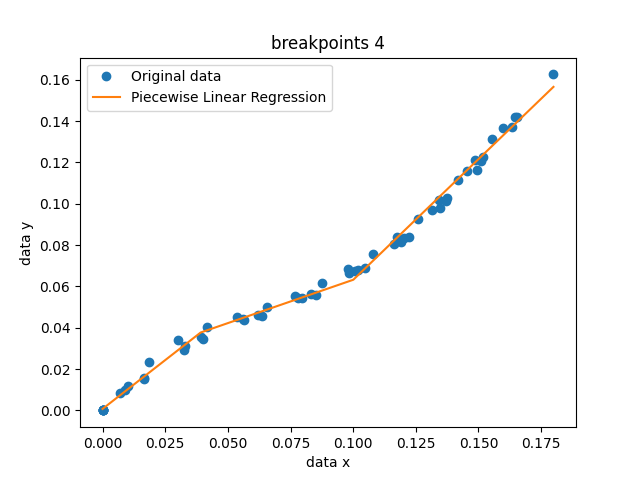
\includegraphics[scale=0.35]{./figure/chapter6/test1/image01.png}
      \label{image01}
     \end{minipage}
    }
       \subfigure[]
       {
        \begin{minipage}{7cm}
         \centering
         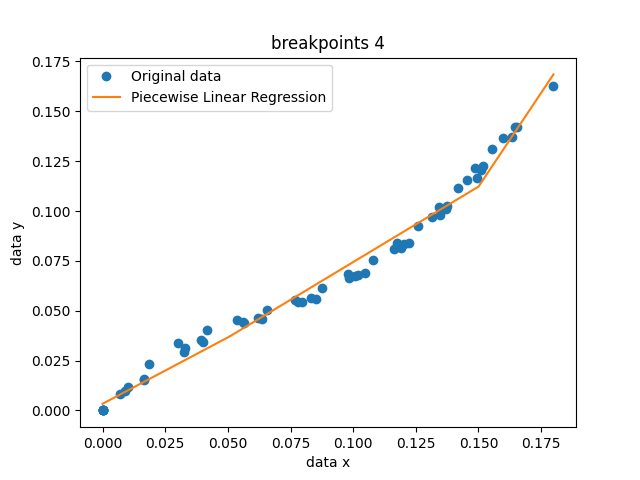
\includegraphics[scale=0.35]{./figure/chapter6/test1/image02.png}
         \label{image02}
        \end{minipage}
       }
   \caption{已知断点位置多段线性回归}
   \label{image0102}
   \end{figure}

同时,上述两种断点位置的分配对应的标准差和判定系数分别为:

\[\begin{aligned}
    SE(\beta_1)=[0.00096346,0.0388971,0.05737514,0.04040854]~
    R^2_1=0.99610201
    \\
    SE(\beta_2)=[0.00175845,0.05263311,0.07186705,0.16834045]~
    R^2_2=0.98563604
    \end{aligned}\]

通过观察上述曲线图像和相关系数可以知道,第一个断点位置分配更优。从这个测试中,我们也可以知道标准差和判定系数可以用于判断分段线性回归的效果。

\subsection{测试2}

使用 PLR 类构建模型,进行已知断点数目位置的多段线性回归。图 \ref{image03} 是分段数为5的运行结果,可以看到拟合曲线表现较不错。

\begin{figure}[H]
    \center{\includegraphics*[width = .8\textwidth]{./figure/chapter6/test2/image03.png}}
    \caption{PLR 模型构建全局最优的断点位置}
    \label{image03}      
\end{figure}

如此还可以继续改变分段的数目,并使用差分进化算法得到全局最佳的断点位置。这种思想在 \nameref{test3} 中得到了体现。


\subsection{测试3\label{test3}}

通过遍历多个分段数,每个分段数都输出拟合曲线的图像。同时生成判定系数随分段数增加而变化的曲线图。以下甄选出了一些典型分段数对应的拟合曲线,如图 \ref{test3} 所示。同时,还绘制了判定系数的变化曲线,如图 \ref{r_squares} 所示。

从图中可以看到,当分段数增加时,虽然标准差和判定系数都会变得更好,但是从图中直观来看,分段数增加到一定数目之后,拟合曲线就会出现毛刺(这一般是不被期望的),也就是说分段数过多会导致数据过拟合的情况,因此并不是分段数越多越优。

从判别系数随分段数变化曲线也可以看到,开始时,判别系数随分段数增加而显著增加;而当分段数增加到一定量后继续增加时,判别系数增加速度显著下降,并逐渐趋近$1$。以上测试结果对我们实际应用中的启示是,应该选择合适的分段数使得各种判定的数值足够优秀且避免数据过拟合的情况。

\begin{figure}[H]
    %\begin{tabular}{cc}   
    \begin{minipage}{0.48\linewidth}
      \centerline{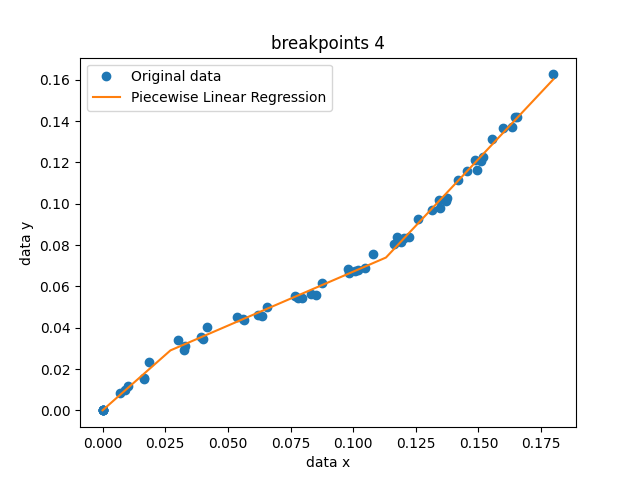
\includegraphics[width=8.0cm]{./figure/chapter6/test3/segment03.png}}
      \centerline{(a) segment 3}
    \end{minipage}
    \hfill
    \begin{minipage}{.48\linewidth}
      \centerline{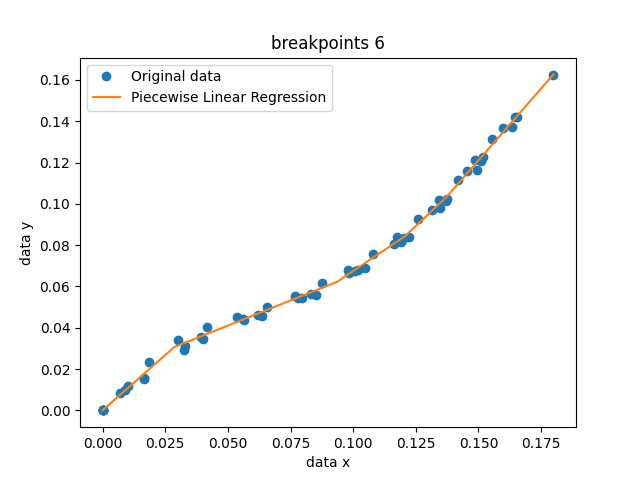
\includegraphics[width=8.0cm]{./figure/chapter6/test3/segment05.png}}
      \centerline{(b) segment 5}
    \end{minipage}
    \vfill
    \begin{minipage}{0.48\linewidth}
      \centerline{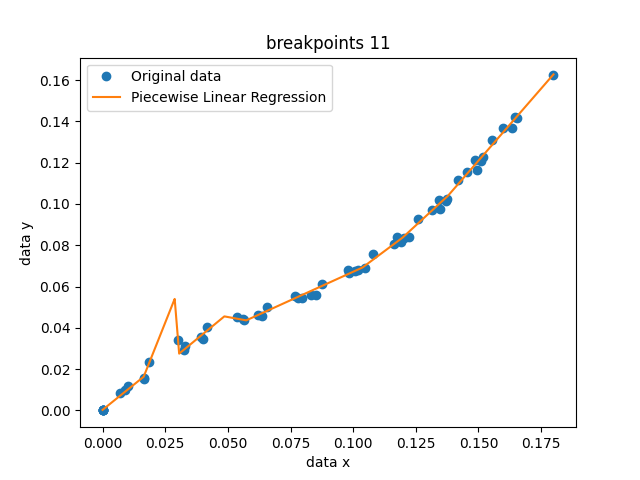
\includegraphics[width=8.0cm]{./figure/chapter6/test3/segment10.png}}
      \centerline{(c) segment 10}
    \end{minipage}
    \hfill
    \begin{minipage}{0.48\linewidth}
      \centerline{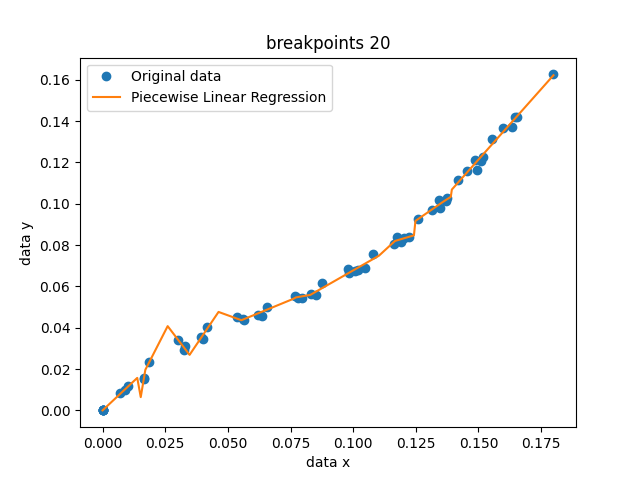
\includegraphics[width=8.0cm]{./figure/chapter6/test3/segment19.png}}
      \centerline{(d) segment 19}
    \end{minipage}
    %\end{tabular}
    \caption{各种不同分段数对应的线性拟合}
    \label{test3}
\end{figure}

\begin{figure}[H]
    \center{\includegraphics*[width = .6\textwidth]{./figure/chapter6/test3/r_squares.png}}
    \caption{判别系数随分段数增加的变化}
    \label{r_squares}      
\end{figure}

\subsection{测试4\label{test4}}

测试差分进化算法的收敛速度。这个测试对不同维数的数据,根据相同的评价函数,得到评价函数的最小值与迭代次数之间的关系如图 \ref{diffe} 所示。

\begin{figure}[H]
    \center{\includegraphics*[width = .7\textwidth]{./figure/chapter6/test4/de.png}}
    \caption{判别系数随分段数增加的变化}
    \label{diffe}      
\end{figure}

从图中可以看出,随着数据维数不断提高,差分进化算法收敛至全局最优点的迭代数不断增加。正如前文 \nameref{p2} 提到的,差分进化算法的收敛速度事实上随着维数的增加而呈指数型增加的趋势。所以,面对维数较大的数据集,比如Facebook 的经典评论数据集($54$维),该算法很可能开销难以容忍。

\subsection{测试5}

对于给定的实例数据集,通过 PLR 类建立模型,考察差分进化算法的收敛速度。这个测试与 \nameref{test4} 异曲同工,只是数据集更加具有普适性和一般性。测试的收敛速度如图 \ref{diffe_real} 所示。

从图中可以看出,该测试结果与 \nameref{test4} 显著不同,对于不同分段数,其最后收敛的值不同,原因是,对于一个真实数据集,不同分段数作用于数据集的效果是不同的。这也为我们找到全局最优分段数提供了思路,我们可以找到具有最小收敛$SS_{res}$值的分段数作为全局最优分段数。但是,这样的想法也是有问题,因为如果$segment = n$,则$SS_{res}$将等于$0$。

\begin{figure}[H]
    \center{\includegraphics*[width = .7\textwidth]{./figure/chapter6/test5/de_real.png}}
    \caption{判别系数随分段数增加的变化}
    \label{diffe_real}      
\end{figure}

回到图像本身,对于不同的分段数,算法收敛的速度是不一样的,一个显而易见的结论是,最终收敛值越小,所需的迭代次数越多。当然,这其中也有反例,比如segment7的收敛速度比segment6收敛速度快。因为本实验中采用$rand/1/bin$的策略,所以每次运行的结果也都是不同的。


\subsection{测试6}

这个测试中,观察分段线性回归模型对于非多项式函数的拟合情况。采用不同分段数对数据集进行拟合。结果如图 \ref{test6} 所示。其中源数据是从函数$y=cosx$进行偏置震荡得来的,如图 \ref{poly2} 所示;拟合曲线如图 \ref{poly1} 所示。

从图中可以看到,不同分段数对应的拟合曲线差别不大。也就是说,在分段数不大的情况下,拟合的曲线就已经可以反映数据集的大致分布。这给我们的启发是,在实际运用多段线性回归时,不一定需要选择较大的分段数或者全局最优分段数,在较小的分段数下,我们就可以得到曲线的大致分布,并且开销较小(差分进化算法开销随维数增加而指数型增加)。

\begin{figure}[H]
    \centering
    \subfigure[]
    {
     \begin{minipage}{7cm}
      \centering
      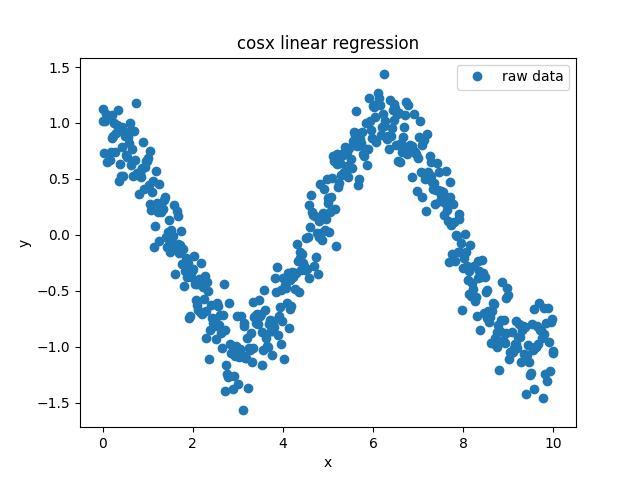
\includegraphics[scale=0.35]{./figure/chapter6/test6/poly2.png}
      \label{poly2}
     \end{minipage}
    }
       \subfigure[]
       {
        \begin{minipage}{7cm}
         \centering
         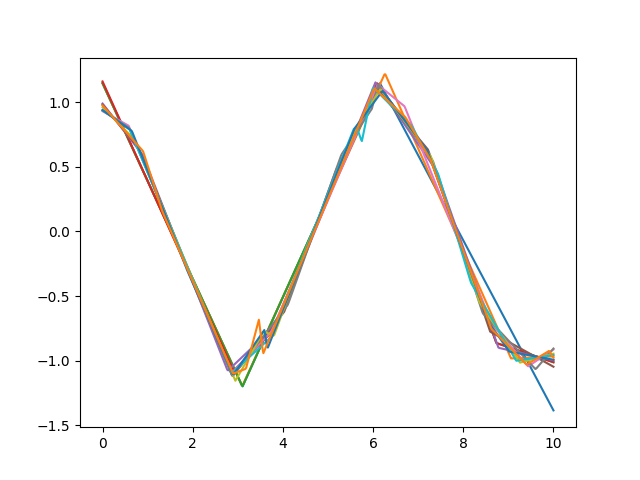
\includegraphics[scale=0.35]{./figure/chapter6/test6/poly1.png}
         \label{poly1}
        \end{minipage}
       }
   \caption{非多项式数据集拟合}
   \label{test6}
   \end{figure}

\subsection{应用结果}

分段线性回归的应用场景非常丰富,本次实验选取股票走势拟合进行简单的应用。首先,使用baostock第三方库调取的上证指数数据可视化后如图 \ref{app1} 所示。观察数据的大致走势,设置好一些列待检的分段数,使用 PLR 类建立模型并进行训练,每个分段数对应的分段函数如 \ref{app2} 图所示。

\begin{figure}[H]
    \center{\includegraphics*[width = 1\textwidth]{./figure/chapter6/app/app1.jpg}}
    \caption{真实数据:上证指数}
    \label{app1}      
\end{figure}

从图上可以看出,拟合的大致效果还是不错的,基本上可以反映出上证指数的走势情况。

\begin{figure}[H]
    \center{\includegraphics*[width = 1\textwidth]{./figure/chapter6/app/app2.jpg}}
    \caption{实际应用:股票拟合}
    \label{app2}      
\end{figure}


综上所示,本次实验的目的已经达到。面对一个数据集,如果在观察到可以使用多段线性回归来对模型进行拟合的情况下,我们可以选用本次使用中使用的方法。首先是对问题进行建模,通过源数据生成回归矩阵,将多段线性回归问题转换成单一线性回归问题,再使用差分进化算法来对残差平方和进行全局优化得到全局最优的$\beta$参数,即断点的位置。

\section{结果分析}
\subsection{环境}


\subsection{系统功能需求}


\subsection{系统设计}


\subsection{系统实现}


\subsection{系统测试及结果说明}


\subsection{其他需要说明的问题}
-
\section{机器学习课程的学习体会与建议}
\subsection{环境}


\subsection{系统功能需求}


\subsection{系统设计}


\subsection{系统实现}


\subsection{系统测试及结果说明}


\subsection{其他需要说明的问题}
%============= 参考文献 =====================
\addcontentsline{toc}{section}{参考文献}
\begin{thebibliography}{99}  
\bibitem{ref1} James F. Kurose, Keith W. Ross. 计算机网络: 自顶向下方法 (第7版) [M]. 机械工业出版社, 2018.
\end{thebibliography}
\clearpage
%=============  致谢  ======================
\newpage
\appendix

\section{附录 I}



\end{document}
%%%%%%%%%% 结束 %%%%%%%%%%